\documentclass[polish, 11pt, a4paper]{article}

\usepackage{polski}
\usepackage[utf8]{inputenc}
\usepackage[autostyle]{csquotes}
\DeclareQuoteAlias{dutch}{polish}
\usepackage[T1]{fontenc}
\usepackage{geometry}
\geometry{
	a4paper,
	total={170mm,257mm},
	left=25mm,
	right=25mm,
	top=20mm,
}

\usepackage{babel}
\usepackage{microtype}
\usepackage{lmodern}
\usepackage{multirow}
\usepackage{array}
\newcolumntype{?}[1]{!{\vrule width #1}}
\usepackage{siunitx}
\usepackage{amsmath}
\usepackage{caption}
\usepackage{graphicx}
\usepackage{graphics}
\usepackage{float}
\usepackage{enumitem}
\usepackage{ragged2e}
\usepackage{parskip}
\RaggedRightParindent=24pt
\usepackage{indentfirst}
\usepackage[figurename=Wykres]{caption}

\begin{document}
	\begin{titlepage}
		\centering
		\Huge Laboratorium Podstaw Fizyki\\
		\vspace{1cm}
		\huge Ćwiczenie 54 \enquote{Badanie zjawiska rezonansu elektromagnetycznego}\\
		\vspace{1cm}
		\raggedright
		\huge Prowadzący: mgr Karolina Paradowska\\
		\vspace{.5cm}
		\begin{table}[h]
			\centering
			\resizebox{\columnwidth}{!}{%
			\begin{tabular}{|r|l|}\hline
				Imię i Nazwisko	&Marcin Kotas\\\hline
				Nr indeksu		&235098\\\hline
				Wydział			&Elektroniki\\\hline
				Termin zajęć	&21.11.2017, godz. 9.15\\\hline
				Numer grupy ćwiczeniowej&5\\\hline
				Data oddania sprawozdania&28.11.2017\\\hline
			\end{tabular}%
			}
		\end{table}
	\end{titlepage}

	\section{Wstęp teoretyczny}
		\RaggedRight
		Celem ćwiczenia było wykreślenie charakterystyki prąd-częstotliwość szeregowego obwodu RLC, wyznaczenie częstotliwości rezonansowej oraz współczynnika dobroci badanego obwodu.
		W tym celu użyty został następujący układ:
		\begin{figure}[H]
			\centering
			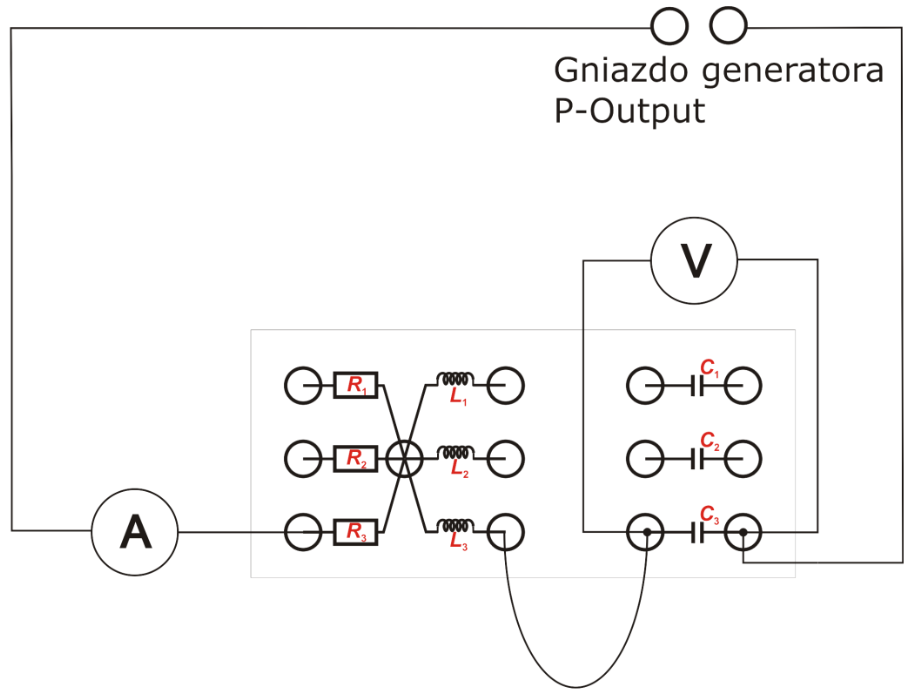
\includegraphics[width=.5\textwidth]{Fizyka54Rysunek1}

			Schemat przedstawiający układ pomiarowy.\\
			Użyto opornika \(R_3\), cewki \(L_3\), oraz kondensatora \(C_3\).
		\end{figure}

		Pojemność kondensatora wyznacza się z następującego wzoru:
		\begin{equation}
			C	=	\frac{1}{(2\pi f_r)^2L}
		\end{equation}
		
		Dobroć obwodu wyznacza się na podstawie następującego wzoru:
		\begin{equation}
			Q=\frac{U_C}{U_0}=\frac{f_r}{\Delta f}
		\end{equation}
	\section{Wyniki pomiarów}

	\subsection{Wykonanie pomiarów}
		Napięcie na generatorze ustawione zostało ustawione na wartość \(300mVrms\), co odpowiada napięciu wyjściowemu w układzie RLC \(U_0=3V\).
		Układ został połączony z użyciem zestawu \(R_3, L_3, C_3\).
		Pomiary zostały wykonane przy stałej wartości napięcia \(U_0\).
		
		Najpierw zmierzona została częstotliwość rezonansowa, która wyniosła \(f_r=1,670kHz\).
		Natężenie prądu dla tej częstotliwości wyniosło \(I_r=9,44mA\), a napięcie na kondensatorze \(U_C=3,56V\).
		Następnie zmierzona została cała charakterystyka prądowa układu dla częstotliwości od \(0,001kHz\) do \(30,0kHz\).
		
		Częstotliwość na generatorze zmieniana była tak, aby w pobliżu częstotliwości rezonansowej punkty pomiarowe były zagęszczone.
		Od \(1,2 kHz\) do \(2,3kHz\) częstotliwość zmieniana była co \(20Hz\), natomiast w pozostałych zakresach zmieniana była co \(50Hz\) lub \(100Hz\).
		Powyżej \(4kHz\) wraz ze wzrostem częstotliwości odległości między pomiarami zwiększane były tak, aby uzyskać pełen obraz krzywej rezonansowej.
		Częstotliwość, dla której prąd zmalał do \(0,10mA\) wyniosła \(30kHz\). Wyniki wszystkich pomiarów umieszczone zostały w Tabelach 1 i 2.
	
	\subsection{Obliczenia}

	\subsubsection{Opracowanie wyników}
		Najpierw sporządzony został wykres całej krzywej rezonansowej (Wykres 1).
		Następnie w celu zwiększenia czytelności wykonany został wykres dla mniejszego zakresu częstotliwości (Wykres 2).
		Na tym wykresie zaznaczona została częstotliwość rezonansowa \(f_r\) oraz natężenie prądu \(I_r\).
		Dla wybranych punktów zaznaczone zostały słupki błędów. Wykres 3 przedstawia przybliżenie wykresu w pobliżu częstotliwości rezonansowej z zaznaczonymi słupkami błędów.
		Wartości słupków błędów równe są błędom pomiarowym użytych przyrządów.
		
		Błąd pomiarów częstotliwości obliczony został według wzoru \((1\%rdg+1 dgt)^{[1]}\), a natężenia prądu według wzoru \((2,5\%rdg+3dgt)\). Na przykładzie pomiaru nr.43:
		\begin{align*}
			\Delta f &= 0,01\cdot 1,72 + 1\cdot 10^{-6} = 0,017201 [kHz]\\
			\Delta I &= 0,025\cdot 8,13 + 0,03 = 0,23325 [mA]			
		\end{align*}
		Indukcyjność cewki \(L_3=(33,0\pm 3,3)mH\).
		Niepewność tych pomiarów to niepewność typu B:
		\begin{align*}
			u(f)&=\frac{\Delta f}{\sqrt{3}} = \frac{0,017201}{\sqrt{3}} = 0,009931002 \approx 0,010 [kHz]\\[6pt]
			u(I)&=\frac{\Delta I}{\sqrt{3}} = \frac{0,23325}{\sqrt{3}} = 0,13466695 \approx 0,14 [mA]\\[6pt]
			u(L)&=\frac{\Delta L}{\sqrt{3}} = \frac{3,3}{\sqrt{3}} = 1,905255888 \approx 2,0 [mH]			
		\end{align*}
		Pojemność kondesatora wyznaczona została ze wzoru (1). :
		\begin{align*}
			C	&=	\frac{1}{(2\pi f_r)^2L} = \frac{1}{(2\pi \cdot 1670)^2 \cdot 0,033} = 275,228486\times 10^{-9}  \approx 275 [\mu F]		
		\end{align*}
		Niepewność wyznaczonej pojemności wyniosła:
		\begin{align*}
			u_c(C)	&=	\frac{1}{2\pi^2}\sqrt{\left[ \frac{u(L)}{2 f_r^2 L^2}\right]^2 + \left[ \frac{u(f_r)}{f_r^3 L}\right]^2}
					=	\frac{1}{2\pi^2}\sqrt{\left[ \frac{0,002}{2\cdot 1670^2\cdot 0,033^2}\right]^2 + \left[ \frac{9,7}{1670^3\cdot 0,033}\right]^2}\\[6pt]
					&=	16,9841709\times 10^{-9} \approx 17 [\mu F]					
		\end{align*}
		Na podstawie napięć \(U_0\) oraz \(U_C\) obliczona została dobroć obwodu:
		\begin{displaymath}
			Q_U = \frac{U_C}{U_0} = \frac{3,56}{3,00} = 1,186667 \approx 1,187			
		\end{displaymath}
		Niepewność wartości Q to niepewność złożona:
		\begin{align*}
			u_c(Q_U)	&=	\sqrt{\left[ \frac{u(U_C)}{U_0}\right]^2 + \left[ \frac{U_C}{U_0^2} u(U_0)\right]^2}
					=	\sqrt{\left[ \frac{0,05}{3,00}\right]^2 + \left[ \frac{3,56}{3,00^2}\cdot 0,01\right]^2}\\[6pt]
					&=	0,017129629	\approx 0,018				
		\end{align*}

		Wartość dobroci może również zostać oszacowana na podstawie wykresu \(I(f)\), korzystając z zależności (2). Należy w tym celu wyznaczyć \(\Delta f = f_p - f_l\).
		Jest to różnica częstotliwości, dla których energia drgań jest równa połowie energii maksymalnej występującej dla częstotliwości rezonansowej.
		Ponieważ częstotliwość \(f_p\) znajduje się pomiędzy \(2,55kHz\), a \(2,60kHz\), jej wartość została oszacowana
		- przyjęto, że zależność \(I(f)\) pomiędzy tymi punktami jest w przybliżeniu liniowa.
		\begin{align*}
			I_{r2}	&=	I_r/\sqrt{2} = 6,675088014 \approx 6,675 [mA]	\\[6pt]
			f_l	&\approx 1,1000 [kHz]\\[6pt]
			f_p	&= 2,55+\frac{(6,75-6,675)\cdot (2,6-2,55)}{6,75-6,58} = 2,55+\frac{0,075\cdot 0,05}{0,17} = 2,55 + 0,022059 \approx 2,572 [kHz]\\[6pt]
			\Delta f &= f_p-f_l = 2,572 - 1,1 = 1,472 [kHz]
		\end{align*}
		Dobroć obwodu wyznaczona z częstotliwości wynosi:
		\begin{displaymath}
			Q_f	= \frac{f_r}{\Delta f} = \frac{1,670}{1,472} = 1,13451087 \approx 1,135			
		\end{displaymath}
		Aby wyznaczyć dokładność tej wartości należy wpierw oszacować dokładność wyznaczonej \(\Delta f\).
		Poniważ dokładność \(u(I_r)=0,16mA\), za dokładność \(\Delta f\) przyjęto różnicę częstotliwości odpowiadającej zmianie natężenia prądu o \(0,16mA\) przy częstotliwości \(2,6kHz\):
		\begin{align*}
			u(\Delta f) &= \frac{0,16}{6,75-6,58}(2,6-2,55) = \frac{0,16}{0,17}\cdot 0,05 = 0,047059 \approx 0,048 [kHz]\\[6pt]
			u_c(Q_f)	&=	\sqrt{\left[ \frac{u(f_r)}{\Delta f}\right]^2 + \left[ \frac{f_r}{\Delta f^2} u(\Delta f)\right]^2}
			=	\sqrt{\left[ \frac{9,7}{1472}\right]^2 + \left[ \frac{1670}{1472^2}\cdot 48\right]^2}\\[6pt]
			&=	0,037577226	\approx 0,038		
		\end{align*}
	
	\newpage
    \subsection{Tabele i wykresy}
    
    	\begin{table}[H]
    		\centering
    		\caption{Wyniki pomiarów cz.1}
    		\begin{tabular}{|r|S[table-format=1.6, output-decimal-marker = {,}]|S[table-format=1.6, output-decimal-marker = {,}]|c|c?{.5mm}r|S[table-format=1.4, output-decimal-marker = {,}]|S[table-format=1.4, output-decimal-marker = {,}]|c|c|}\hline
    			&	{\(f\)}	&	{\(u(f)\)}	&	{\(I\)}	&	{\(u(I)\)}	&	&	{\(f\)}	&	{\(u(f)\)}	&	{\(I\)}	&	{\(u(I)\)}	\\
    			{Lp}	&	{\([kHz]\)}	&	{\([kHz]\)}	&	{\([mA]\)}	&	{\([mA]\)}	&	{Lp}	&	{\([kHz]\)}	&	{\([kHz]\)}	&	{\([mA]\)}	&	{\([mA]\)}	\\\hline
    			1	&	0,001000	&	0,000007	&	0,05	&	0,02	&	41	&	1,6800	&	0,0098	&	9,44	&	0,16	\\\hline
    			2	&	0,05000	&	0,00029	&	0,15	&	0,02	&	42	&	1,7000	&	0,0099	&	9,43	&	0,16	\\\hline
    			3	&	0,10000	&	0,00058	&	0,35	&	0,03	&	43	&	1,720	&	0,010	&	9,42	&	0,16	\\\hline
    			4	&	0,15000	&	0,00087	&	0,65	&	0,03	&	44	&	1,740	&	0,011	&	9,41	&	0,16	\\\hline
    			5	&	0,2000	&	0,0012	&	0,95	&	0,04	&	45	&	1,760	&	0,011	&	9,37	&	0,16	\\\hline
    			6	&	0,3000	&	0,0018	&	1,47	&	0,04	&	46	&	1,780	&	0,011	&	9,34	&	0,16	\\\hline
    			7	&	0,4000	&	0,0024	&	2,00	&	0,05	&	47	&	1,800	&	0,011	&	9,32	&	0,16	\\\hline
    			8	&	0,5000	&	0,0029	&	2,55	&	0,06	&	48	&	1,820	&	0,011	&	9,27	&	0,16	\\\hline
    			9	&	0,6000	&	0,0035	&	3,15	&	0,07	&	49	&	1,840	&	0,011	&	9,24	&	0,16	\\\hline
    			10	&	0,7000	&	0,0041	&	3,78	&	0,08	&	50	&	1,860	&	0,011	&	9,19	&	0,15	\\\hline
    			11	&	0,8000	&	0,0047	&	4,43	&	0,09	&	51	&	1,880	&	0,011	&	9,13	&	0,15	\\\hline
    			12	&	0,9000	&	0,0052	&	5,15	&	0,10	&	52	&	1,900	&	0,011	&	9,08	&	0,15	\\\hline
    			13	&	1,0000	&	0,0058	&	5,90	&	0,11	&	53	&	1,920	&	0,012	&	9,01	&	0,15	\\\hline
    			14	&	1,0500	&	0,0061	&	6,28	&	0,11	&	54	&	1,940	&	0,012	&	8,96	&	0,15	\\\hline
    			15	&	1,1000	&	0,0064	&	6,66	&	0,12	&	55	&	1,960	&	0,012	&	8,88	&	0,15	\\\hline
    			16	&	1,1500	&	0,0067	&	7,05	&	0,12	&	56	&	1,980	&	0,012	&	8,83	&	0,15	\\\hline
    			17	&	1,2000	&	0,0070	&	7,43	&	0,13	&	57	&	2,000	&	0,012	&	8,76	&	0,15	\\\hline
    			18	&	1,2200	&	0,0071	&	7,57	&	0,13	&	58	&	2,020	&	0,012	&	8,67	&	0,15	\\\hline
    			19	&	1,2400	&	0,0072	&	7,72	&	0,13	&	59	&	2,040	&	0,012	&	8,62	&	0,15	\\\hline
    			20	&	1,2600	&	0,0073	&	7,85	&	0,14	&	60	&	2,060	&	0,012	&	8,55	&	0,15	\\\hline
    			21	&	1,2800	&	0,0074	&	7,99	&	0,14	&	61	&	2,080	&	0,013	&	8,47	&	0,14	\\\hline
    			22	&	1,3000	&	0,0076	&	8,13	&	0,14	&	62	&	2,100	&	0,013	&	8,40	&	0,14	\\\hline
    			23	&	1,3200	&	0,0077	&	8,26	&	0,14	&	63	&	2,120	&	0,013	&	8,32	&	0,14	\\\hline
    			24	&	1,3400	&	0,0078	&	8,38	&	0,14	&	64	&	2,140	&	0,013	&	8,25	&	0,14	\\\hline
    			25	&	1,3600	&	0,0079	&	8,50	&	0,15	&	65	&	2,160	&	0,013	&	8,16	&	0,14	\\\hline
    			26	&	1,3800	&	0,0080	&	8,61	&	0,15	&	66	&	2,180	&	0,013	&	8,11	&	0,14	\\\hline
    			27	&	1,4000	&	0,0081	&	8,72	&	0,15	&	67	&	2,200	&	0,013	&	7,99	&	0,14	\\\hline
    			28	&	1,4200	&	0,0082	&	8,82	&	0,15	&	68	&	2,220	&	0,013	&	7,94	&	0,14	\\\hline
    			29	&	1,4400	&	0,0084	&	8,90	&	0,15	&	69	&	2,240	&	0,013	&	7,86	&	0,14	\\\hline
    			30	&	1,4600	&	0,0085	&	8,99	&	0,15	&	70	&	2,260	&	0,014	&	7,78	&	0,13	\\\hline
    			31	&	1,4800	&	0,0086	&	9,08	&	0,15	&	71	&	2,280	&	0,014	&	7,71	&	0,13	\\\hline
    			32	&	1,5000	&	0,0087	&	9,14	&	0,15	&	72	&	2,300	&	0,014	&	7,64	&	0,13	\\\hline
    			33	&	1,5200	&	0,0088	&	9,22	&	0,16	&	73	&	2,350	&	0,014	&	7,45	&	0,13	\\\hline
    			34	&	1,5400	&	0,0089	&	9,26	&	0,16	&	74	&	2,400	&	0,014	&	7,27	&	0,13	\\\hline
    			35	&	1,5600	&	0,0091	&	9,31	&	0,16	&	75	&	2,450	&	0,015	&	7,11	&	0,12	\\\hline
    			36	&	1,5800	&	0,0092	&	9,35	&	0,16	&	76	&	2,500	&	0,015	&	6,91	&	0,12	\\\hline
    			37	&	1,6000	&	0,0093	&	9,38	&	0,16	&	77	&	2,550	&	0,015	&	6,75	&	0,12	\\\hline
    			38	&	1,6200	&	0,0094	&	9,41	&	0,16	&	78	&	2,600	&	0,016	&	6,58	&	0,12	\\\hline
    			39	&	1,6400	&	0,0095	&	9,43	&	0,16	&	79	&	2,650	&	0,016	&	6,43	&	0,12	\\\hline
    			40	&	1,6600	&	0,0096	&	9,44	&	0,16	&	80	&	2,700	&	0,016	&	6,28	&	0,11	\\\hline
    		\end{tabular}
    	\end{table}
		\begin{table}[H]
		\begin{minipage}{.5\textwidth}
    		\centering
    		\caption{Wyniki pomiarów cz.2}
    		\begin{tabular}{|r|S[table-format=2.3, output-decimal-marker = {,}]|S[table-format=1.3, output-decimal-marker = {,}]|c|c|}\hline
    			&	{\(f\)}	&	{\(u(f)\)}	&	{\(I\)}	&	{\(u(I)\)}	\\
    			{Lp}	&	{\([kHz]\)}	&	{\([kHz]\)}	&	{\([mA]\)}	&	{\([mA]\)}\\\hline
    			81	&	2,750	&	0,016	&	6,13	&	0,11	\\\hline
    			82	&	2,800	&	0,017	&	5,99	&	0,11	\\\hline
    			83	&	2,850	&	0,017	&	5,85	&	0,11	\\\hline
    			84	&	2,900	&	0,017	&	5,73	&	0,11	\\\hline
    			85	&	2,950	&	0,018	&	5,60	&	0,10	\\\hline
    			86	&	3,000	&	0,018	&	5,46	&	0,10	\\\hline
    			87	&	3,100	&	0,018	&	5,26	&	0,10	\\\hline
    			88	&	3,200	&	0,019	&	5,03	&	0,09	\\\hline
    			89	&	3,300	&	0,020	&	4,85	&	0,09	\\\hline
    			90	&	3,400	&	0,020	&	4,66	&	0,09	\\\hline
    			91	&	3,500	&	0,021	&	4,47	&	0,09	\\\hline
    			92	&	3,600	&	0,021	&	4,34	&	0,08	\\\hline
    			93	&	3,700	&	0,022	&	4,16	&	0,08	\\\hline
    			94	&	3,800	&	0,022	&	4,04	&	0,08	\\\hline
    			95	&	3,900	&	0,023	&	3,88	&	0,08	\\\hline
    			96	&	4,000	&	0,024	&	3,76	&	0,08	\\\hline
    			97	&	4,200	&	0,025	&	3,53	&	0,07	\\\hline
    			98	&	4,400	&	0,026	&	3,33	&	0,07	\\\hline
    			99	&	4,600	&	0,027	&	3,15	&	0,07	\\\hline
    			100	&	4,800	&	0,028	&	2,95	&	0,06	\\\hline
    			101	&	5,000	&	0,029	&	2,78	&	0,06	\\\hline
    			102	&	5,200	&	0,031	&	2,66	&	0,06	\\\hline
    			103	&	5,400	&	0,032	&	2,52	&	0,06	\\\hline
    			104	&	5,600	&	0,033	&	2,37	&	0,06	\\\hline
    			105	&	5,800	&	0,034	&	2,25	&	0,05	\\\hline
    			106	&	6,000	&	0,035	&	2,15	&	0,05	\\\hline
    			107	&	6,500	&	0,038	&	1,87	&	0,05	\\\hline
    			108	&	7,000	&	0,041	&	1,65	&	0,05	\\\hline
    			109	&	7,500	&	0,044	&	1,43	&	0,04	\\\hline
    			110	&	8,000	&	0,047	&	1,25	&	0,04	\\\hline
    			111	&	8,500	&	0,050	&	1,04	&	0,04	\\\hline
    			112	&	9,000	&	0,052	&	0,88	&	0,04	\\\hline
    			113	&	9,500	&	0,055	&	0,74	&	0,03	\\\hline
    			114	&	10,000	&	0,058	&	0,62	&	0,03	\\\hline
    			115	&	15,000	&	0,087	&	0,32	&	0,03	\\\hline
    			116	&	20,00	&	0,12	&	0,21	&	0,03	\\\hline
    			117	&	25,00	&	0,15	&	0,13	&	0,02	\\\hline
    			118	&	30,00	&	0,18	&	0,10	&	0,02	\\\hline
    			
			\end{tabular}
		\end{minipage}%
		\begin{minipage}{.5\textwidth}
			\centering
			\caption{Wyniki działań}
			\begin{tabular}{|r|c|c|}\hline
					&	\(x\)	&	\(u(x)\)	\\\hline
				\(U_0 [V]\)	&	3,00	&	0,01	\\\hline
				\(f_r [kHz]\)	&	1,6700	&	0,0097	\\\hline
				\(I_r [mA]\)	&	9,44	&	0,16	\\\hline
				\(U_C [V]\)	&	3,56	&	0,05	\\\hline
				\(L_3 [mH]\)	&	33,0	&	2,0	\\\hline
				\(C_3 [\mu F]\)	&	275	&	17	\\\hline
				\(Q_U\)	&	1,187	&	0,018	\\\hline
				\(\Delta f [kHz]\)	&	1,472	&	0,048	\\\hline
				\(Q_f\)	&	1,135	&	0,038	\\\hline
			\end{tabular}
		\end{minipage}
    	\end{table}
    	
    	\begin{figure}[H]
    		\centering
    		\caption{Krzywa rezonansowa na całym zmierzonym zakresie}
    		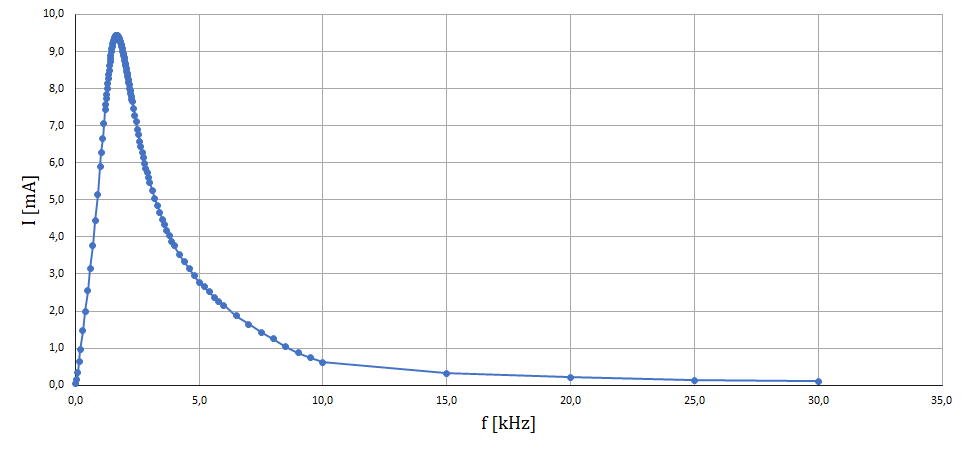
\includegraphics[width=\textwidth]{Fizyka54Wykres1}
    	\end{figure}
    
    	\begin{figure}[H]
    		\centering
    		\caption{Krzywa rezonansowa w zakresie \((0 - 5) kHz\)}
    		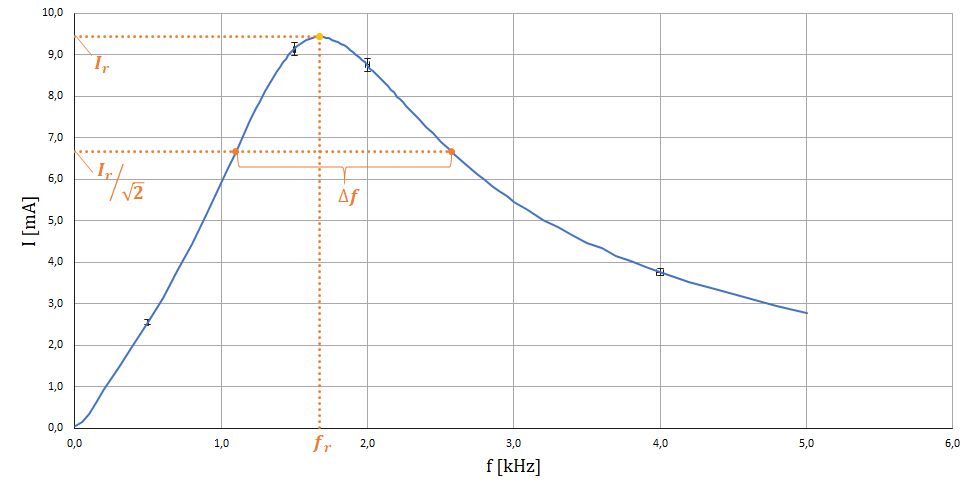
\includegraphics[width=\textwidth]{Fizyka54Wykres2}
    	\end{figure}
    	
    	\begin{figure}[H]
    		\centering
    		\caption{Przybliżenie na słupki błędów przy częstotliwości rezonansowej}
    		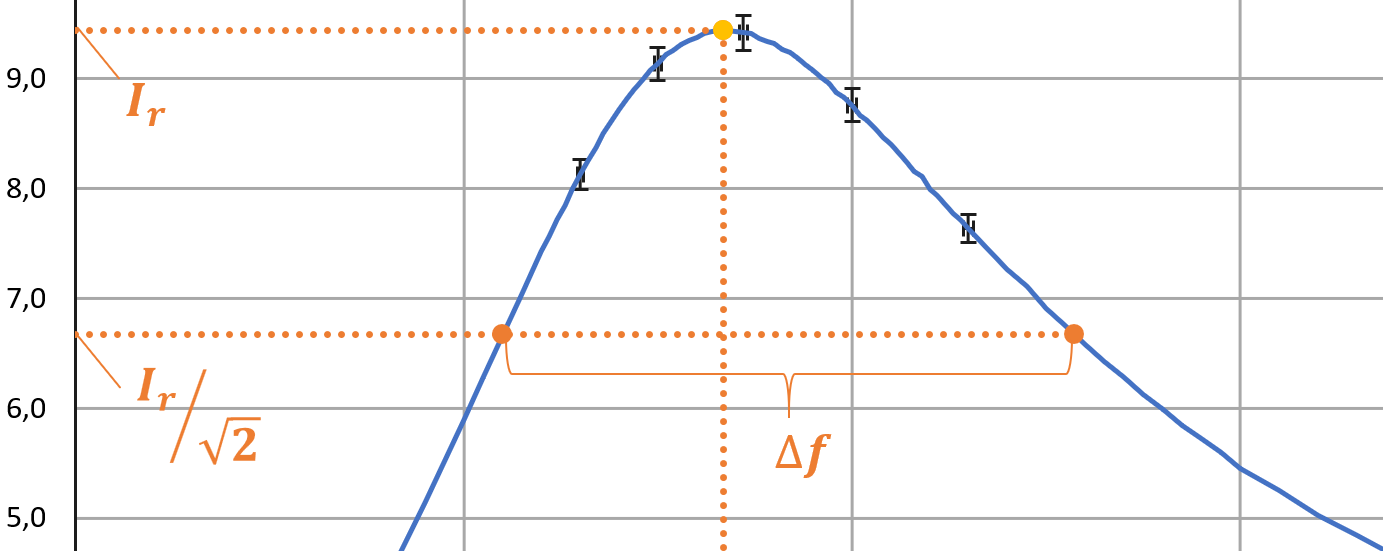
\includegraphics[width=\textwidth]{Fizyka54Wykres3}
    	\end{figure}
    	
	\section{Ostateczne wyniki}
		Ostateczne wyniki wraz z zaokrągleniami:
		\begin{description}[align=right,labelwidth=10cm]
			\item [Częstotliwość rezonansowa:]{\((1,6700\pm 0,0097)kHz\)}
			\item [Pojemność kondensatora:] {\((275\pm 17)\mu F\)}
			\item [Dobroć obwodu wyliczona z napięć:] {\((1,187\pm 0,018)\)}
			\item [Dobroć obwodu wyliczona z częstotliwości:] {\((1,135\pm 0,038)\)}
		\end{description}

	\section{Dyskusja i wnioski}
		Celem ćwiczenia było wyznaczenie pojemności kondensatora, częstotliwości rezonansowej oraz współczynnika dobroci obwodu. 
		Narysowany został wykres charakterystyki prądowej, na którym zaznaczona została częstotliwość rezonansowa.
		Niepewność wyznaczonej częstotliwości jest mniejsza niż 1\%, co wynika z bardzo wysokiej dokładności przyrządu pomiarowego.
		Dobroć obwodu wyliczona z napięć jest dokładniejsza niż ta wyliczona na podstawie częstotliwości, ponieważ \(\Delta f\) musiało zostać oszacowane.

	\section{Literatura}
		\begin{enumerate}[label={[\arabic*]}]
			\item \enquote{można wziąć tam nie wiem, 1\% i bedzie spoczko} - mgr Karolina Paradowska,\\
			źródło: https://www.facebook.com/groups/1010700165711416/permalink/1518896528225108/
		\end{enumerate}

\end{document}